\newpage 

\section{Shortest Paths - Bellman-Ford Algorithm}
Revisiting the shortest path problem (\ref{sec:dstra}), Dijkstra's failed to 
account for negative edge weights. This was a result of fixing nodes too early in the algorithm,
as it assumes paths can only get larger beyond each point. We look to correct this by considering all possible paths from the source node.
\begin{theo}[Bellman-Ford Algorithm]

    \label{theo:bellman}
    Given a connected graph $G$ with $n$ nodes and a source node $s$, begin with setting 
    every node's distance as $\infty$ and $s$ as 0. Keep a parent-child list to build our solution. Let $d(v):=$ ``current distance of $s\to v$,'' and 
    $w(v,u):=$ ``edge-weight $v\to u$.'' Then, for $n-1$ iterations:
    \begin{enumerate}
        \item [(i.)] Iterate over all nodes $v\in G$ starting with $s$.
        \item [(ii.)] For each $v$, iterate out-degrees $u$, and evaluate $w(v,u)$.
        \item [(iii.)] If $d(v)+w(v,u)<d(u)$, update $d(u)=d(v)+w(v,u)$.
        \item [(iv.)] Update parent-child list with $u$ as child of $v$.
    \end{enumerate}
\end{theo}
\noindent
Say we start with $s$, and examine all out-degrees $u$. We update their distances $d(s)+w(s,u)$. Now all $u$ nodes 
have a distance to contribute to their out-degrees. As hash-tables are unordered it is possible we reach a node $d(v)=\infty$, 
before an in-degree of $v$ updates it. If such happens we skip the node, as it is not reachable from $s$.\\

\noindent
Thus using the idea that the sub-paths of the shortest path are also shortest paths, we gather that
each iteration a new shortest path is found. This allows us to find newer shortest paths.
\begin{figure}[h]
    \centering
    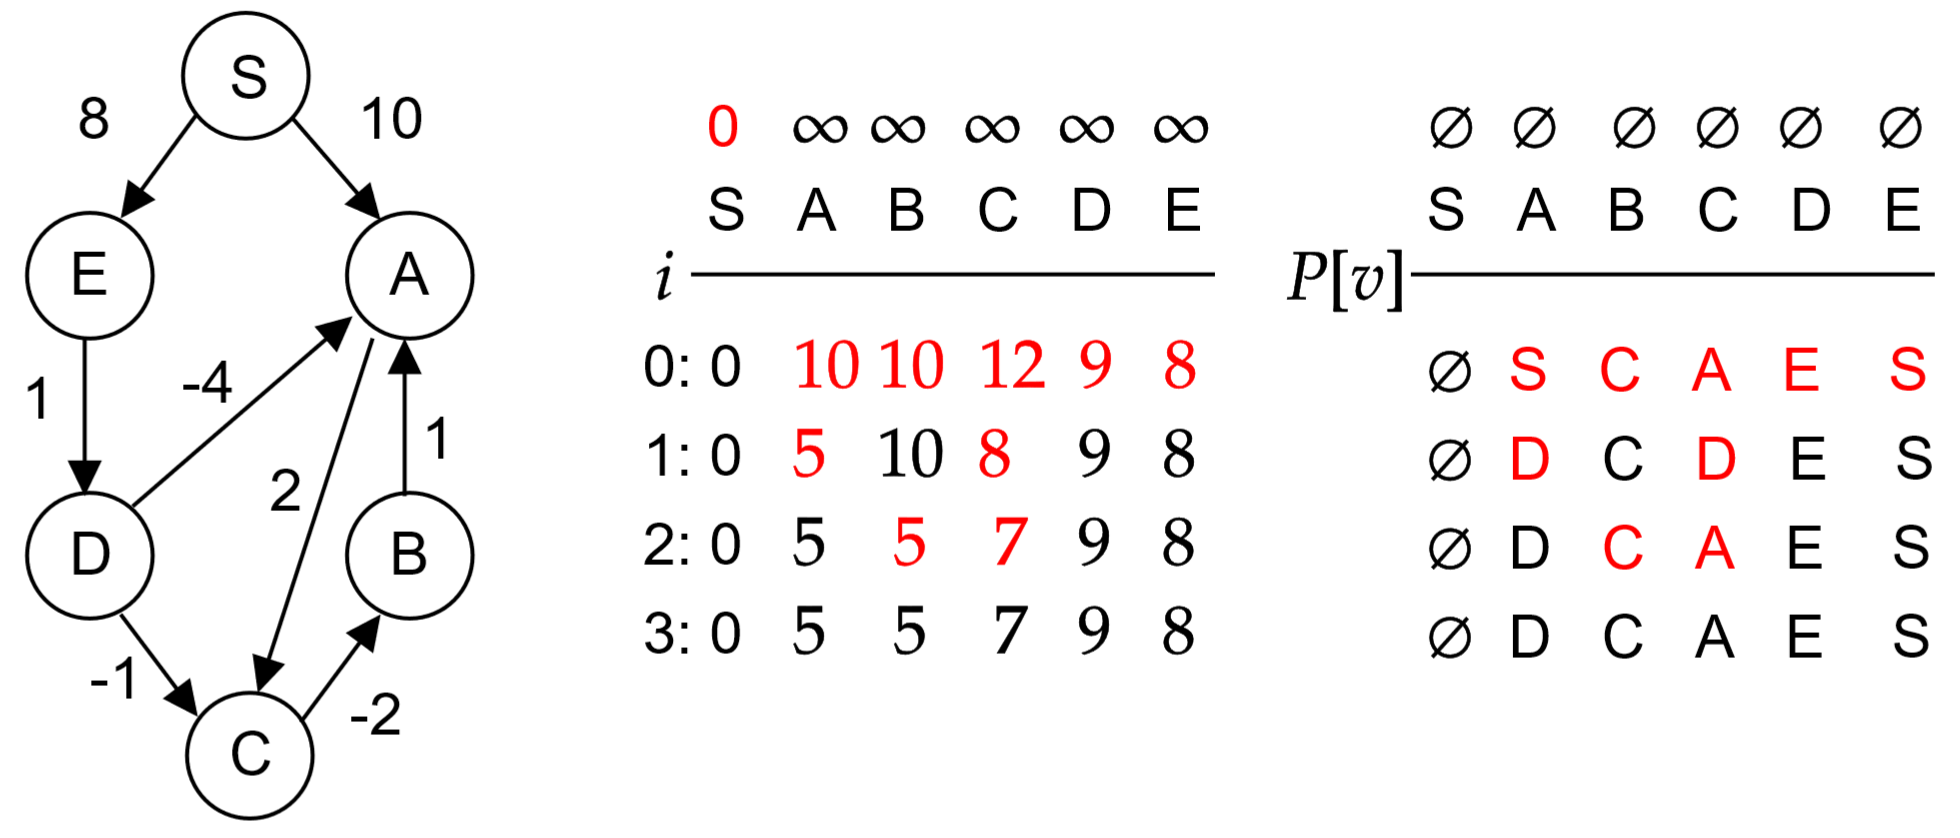
\includegraphics[width=0.8\textwidth]{Sections/dp/bford.png}
    \caption{Bellman-Ford Algorithm, where $i$ depicts iterations and $P[v]$ parents of $v$.}
    \label{fig:bford}
\end{figure}

\vspace{-1em}
\begin{Tip}
    Bellman-Ford Alg. Live Demo: \url{https://www.youtube.com/watch?v=obWXjtg0L64}.
\end{Tip}
\newpage 

\noindent
Our first iteration goes as follows, $d(S)=0$. We check \underline{$min\{\text{evaluation weight},\text{current weight}\}$.}
\begin{itemize}
    \item \textbf{S:}
    \vspace{-2em}
    \begin{itemize}
        \item [] $d(S)+w(S,A)=0+10; d(A)\gets min\{10,\infty\}$
        \item [] $d(S)+w(S,E)=0+8; d(E)\gets min\{8,\infty\}$
    \end{itemize}
    \item \textbf{A:}
    \vspace{-2em}
    \begin{itemize}
        \item [] $d(A)+w(A,C)=10+2; d(C)\gets min\{12,\infty\}$
    \end{itemize}
    \item \textbf{B:} \hspace{.5em} $d(B)=\infty$, currently unreachable from $S$; skip.
    \item \textbf{C:}
    \vspace{-2em}
    \begin{itemize}
        \item [] $d(C)+w(C,B)=12+(-2); d(B)\gets min\{10,\infty\}$
    \end{itemize}
    \item \textbf{D:} \hspace{.5em} $d(D)=\infty$, currently unreachable from $S$; skip.
    \item \textbf{E:}
    \vspace{-2em}
    \begin{itemize}
        \item [] $d(E)+w(E,D)=8+1; d(D)\gets min\{9,\infty\}$.
    \end{itemize}
\end{itemize}
\noindent
Notice how in the second iteration in Figure (\ref{fig:bford}), $A$ and $C$ are updated as a direct consequence of us now being 
able to evaluate paths leaving $D$. This insight gives us the following theorem:

\begin{theo}[Bellman-Ford Alg. - Early Termination]

    We may end the algorithm early if no updates are made in an iteration, as there are no new shortest paths to evaluate.
\end{theo}
\noindent
Though just like Dijkstra's algorithm, Bellman-Ford also has an Achilles' heel. If a negative cycle exists, the algorithm will 
loop indefinitely, as there will always be a new shortest path. Moreover on the next page.

\begin{Def}[Negative Cycle]

    A negative cycle is a cycle whose total weight is negative.
\end{Def}

\noindent
Below find the shortest path from $a\to c$:
\begin{figure}[h]
    \centering
    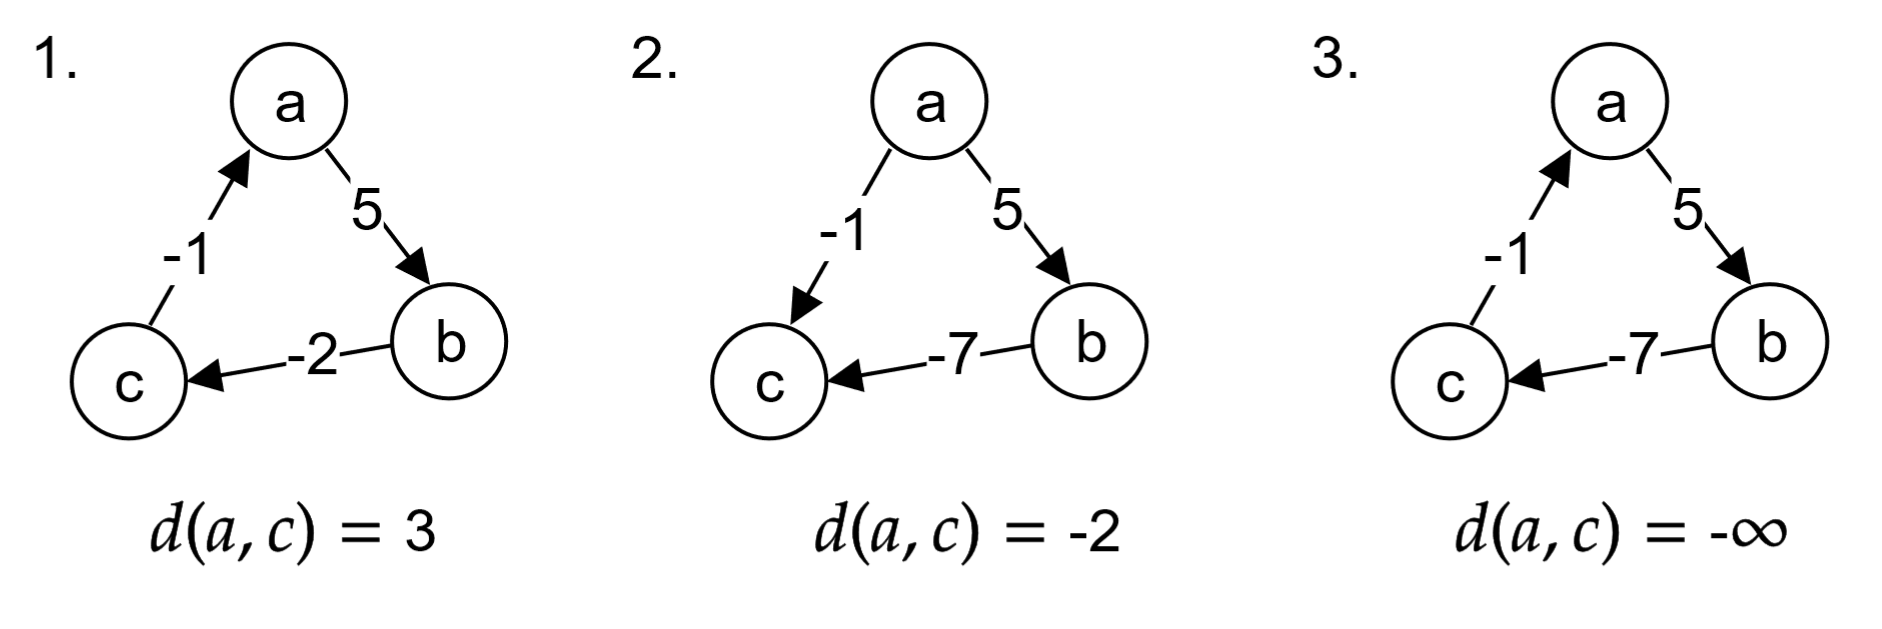
\includegraphics[width=0.8\textwidth]{Sections/dp/negcyc.png}
    \caption{Three graphs: 1. A positive cycle, 2. A DAG, 3. A negative cycle.}
    \label{fig:ncycle}
\end{figure}

\noindent
Examining 3. in Figure (\ref{fig:ncycle}), if we run Bellman-Ford on this graph, we will continuously find a new shortest path to $c$.
We then update the shortest path for $a\to c$, subsequently updating a new shortest path $a\to b$, and so on.
\begin{theo}[Bellman-Ford Alg. - Negative Cycle Detection]

    To detect a negative cycle, run Bellman-Ford for $n-1$ iterations. If a new shortest path is found in the last iteration, a negative cycle exists. As by then,
    we should have solidified a solution.
\end{theo}
\noindent
We identify the choices we make in Figure (\ref{fig:bford})'s routine into a recursive formula:
\[
OPT(i, v) = 
\begin{cases} 
0 & \text{if } i = 0 \text{ and } v = s, \\ 
+\infty & \text{if } i = 0 \text{ and } v \neq s, \\
\min \left\{ 
\begin{array}{l}
OPT(i - 1, v), \\
\min\limits_{u \in G(v)} \left( OPT(i - 1, u) + w(u, v) \right)
\end{array} 
\right\} & \text{if } i > 0.
\end{cases}
\]
% \noindent
% For reference we provide Figure (\ref{fig:bford}) once more:
% \begin{figure}[h]
%     \centering
%     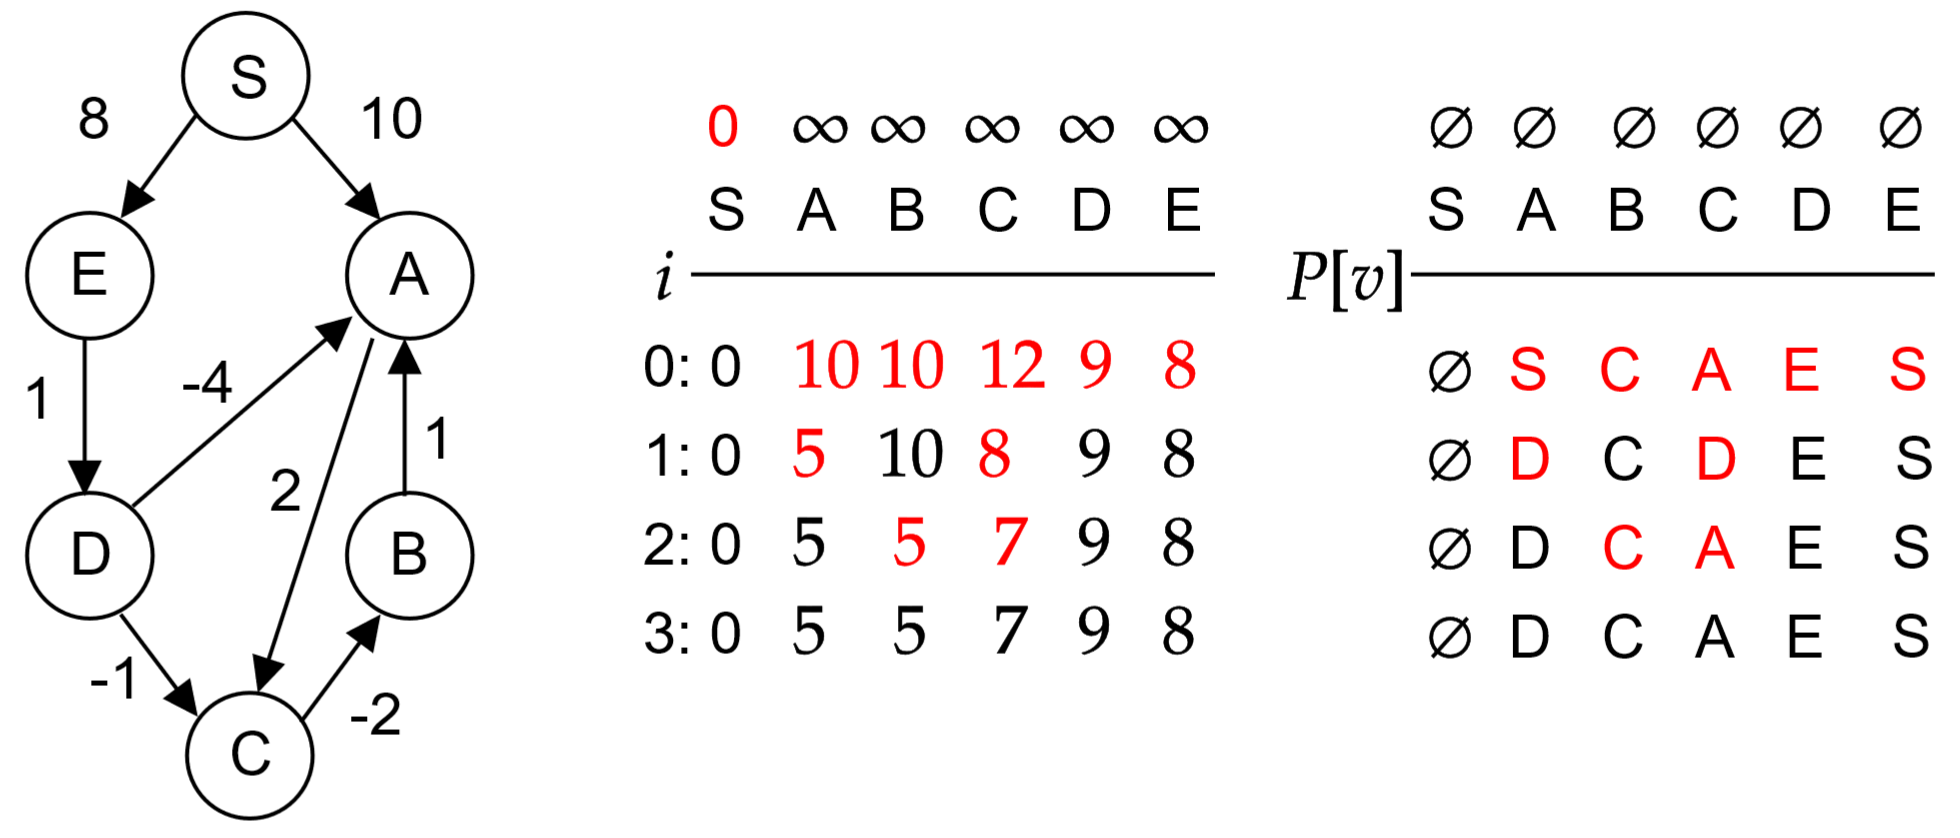
\includegraphics[width=0.7\textwidth]{Sections/dp/bford.png}
%     \caption{Bellman-Ford Algorithm, where $i$ depicts iterations and $P[v]$ parents of $v$.}
% \end{figure}

\noindent
Say we are evaluating node $v$. We first take the last iteration's shortest path $d(v)$ and compare it to possible paths $d'$. To 
find such $d'$ we iterate over all in-degrees $u\to v$ and see if $d(u)+w(u,v)<d(v)$. If so, we update $d(v)=d(u)+w(u,v)$.\\

\noindent
In figure (\ref{fig:bford}) we see on our second iteration, $A$ and $C$ are updated upon evaluating their new in-degree $D$.
Below is pseudo-code for the Bellman-Ford algorithm, returning a DP table $M$ and a parent list $parents$.
\begin{Func}[Bellman-Ford - \textit{BellmanFord()}]

    \vspace{-.5em}
    \begin{algorithm}[H]
        \SetKwProg{Fn}{Function}{:}{}
        $G \gets \text{Graph}$ \tcp{Graph $G$ with $n$ nodes}
        $parents \gets \text{length-}n \text{ table}$ \tcp{Parents list for shortest paths tree}
        
        $M \gets n \times n$ table \tcp{DP table $M[i][v] = OPT(i, v)$}
        $M[0][*] \gets \infty$ \tcp{Set all base values}
        $M[0][s] \gets 0$ \tcp{Base case for source}
        
        \For{$i \gets 1$ \KwTo $n - 1$}{
            \For{$v \in G$}{
                $M[i][v] \gets M[i-1][v]$; \tcp{Copy previous iteration}
                
                \For{$u \in G[v]$}{
                    \If{$M[i-1][u] > M[i][v] + G[v][u]$}{
                        $M[i][u] \gets M[i][v] + G[v][u]$\;
                        $parents[u] \gets v$\;
                    }
                }
            }
        }
        
        \Return $M, \; parents$\;
    \end{algorithm}
    
    \noindent
    \rule{\textwidth}{0.4pt}
    \textbf{Time Complexity:} $O(nm)$. We iterate $n-1$ times for $n+m$ edges. Then $O(n(n+m))=(n^2 + nm)$; however,
    even in tree structures $m=n-1$. So here $m$ could be much larger, s.t., $m\geq n$. Therefore, $nm$ dominates $n^2$
    in the expression. Hence, $O(nm)$.
\end{Func}
\noindent
Let's again examine the above Figure at $i=1$. Say we reach line 7, with $v=D$. We then copy it's previous iteration,
9, and iterate over it's out-degrees $u$. We reach $u=A$, where $M[i-1][A]=10$ and $M[i][D]=9$. We see $10>9+(-4)$,
and update $M[i][A]=5$ and update $parents[A]=D$.

